%%%%%%%%%%%%%%%%%%%%%%%%%%%%%%%%%%%%%%%%%%%%%%%%%%%%%%%
% % Lines starting with % are comments, which are ignored.
% % This is a handy way of indicating the date and version of
% % your document, to wit:
% %
% % LaTeX sample file
% % Modified March, 2002
% %
%%%%%%%%%%%%%%%%%%%%%%%%%%%%%%%%%%%%%%%%%%%%%%%%%%%%%%%
\DocumentMetadata{
  % PDF standards: ONE key whose value is a comma-separated list --
  % UA-2 (accessibility) plus A-4f (archival; the archival companion of
  % UA-2). Do NOT use separate pdfstandard=... keys: with ordinary
  % key-value parsing only the last one takes effect.
  pdfstandard={UA-2,A-4f},
  lang=en-US,
  tagging=on,
  tagging-setup={
    math/setup=mathml-SE
  }
}

\documentclass[12pt]{exam}
% worksheet-macros.tex -- shared package setup for worksheet-template.tex.
%
% NOTE ON PATHS: every template in this repository is stored one level up
% from where it is compiled (see README.md). All relative \input paths
% below are resolved against the folder the document is compiled in,
% which sits one directory above this file.

% --- Math ------------------------------------------------------------
% amsmath: equation environments and numbering
% amsfonts: \mathbb etc.  |  mathrsfs: \mathfrak  |  stmaryrd: extra symbols
\usepackage{amsmath}
\usepackage{amsfonts}
\usepackage{mathrsfs}
\usepackage{stmaryrd}

% --- Layout and glyphs ------------------------------------------------
% float: [H] float placement (stop floats where you put them)
% fontspec: Unicode/OpenType fonts (compile with XeLaTeX or LuaLaTeX)
% emoji: emoji glyphs in the text
\usepackage{float}
\usepackage{fontspec}
\usepackage{emoji}

% --- Typography --------------------------------------------------------
% Atkinson Hyperlegible as the document-wide sans serif (sfdefault):
% a high-legibility face that is easier to read for students with
% dyslexia or low vision.
\usepackage[sfdefault]{atkinson}

% --- Colors -------------------------------------------------------------
% dvipsnames: extended named color palette (the Accessible* colors in
%   lecture-macros.tex are built on it);
% table: \rowcolors / \cellcolor for shading worksheet tables.
% NOTE: xcolor may only be loaded ONCE per document -- a second
% \usepackage{xcolor} with different options is a fatal "Option clash"
% error, so ALL of its options are listed here.
\usepackage[dvipsnames,table]{xcolor}

% --- Multimedia ---------------------------------------------------------
% animate: embeds audio/video (and legacy Flash) media in the worksheet.
\usepackage{animate}

% --- Bibliography --------------------------------------------------------
% biblatex (biber backend): citations and a reference list for worksheets.
\usepackage[
  backend=biber,
  style=alphabetic,
  url=true,
  doi=true,
  isbn=true,
  backref=true
]{biblatex}

% --- Links ---------------------------------------------------------------
% hyperref makes every \ref/citation/URL clickable in the PDF.
% Link colors must satisfy WCAG 1.4.3 (>= 4.5:1 contrast on white):
%   blue = 8.6:1, green!40!black = 7.2:1.
% (The old cyan/magenta values measured 1.25:1 / 3.1:1 and failed.)
\usepackage{hyperref}
\hypersetup{
  colorlinks=true,
  linkcolor=blue,
  filecolor=blue,
  urlcolor=green!40!black,
}

% --- Shared course macros ------------------------------------------------
% Root macros.tex: math shorthands used across all course documents
% (\RR, \NN, \ZZ, \QQ, \grad, \curl, \tr, \der, \pder, ...).
\newcommand{\RR}{\mathbb{R}}
\newcommand{\NN}{\mathbb{N}}
\newcommand{\ZZ}{\mathbb{Z}}
\newcommand{\QQ}{\mathbb{Q}}
\newcommand{\vv}{\vec{v}}
\newcommand{\ww}{\vec{w}}
\newcommand{\xx}{\vec{x}}
\newcommand{\yy}{\vec{y}}
\newcommand{\zz}{\vec{z}}
\newcommand{\uu}{\vec{u}}
\newcommand{\basis}[1]{\vec{e_{#1}}}
\newcommand{\id}{\mathrm{id}}
\newcommand{\CC}{\mathbb{C}}
\renewcommand{\div}{\operatorname{div}}
\newcommand{\grad}{\operatorname{grad}}
\newcommand{\curl}{\operatorname{curl}}
\newcommand{\tr}{\operatorname{tr}}
\newcommand{\der}[2]{\dfrac{d #1}{d #2}}
\newcommand{\pder}[3][]{\dfrac{\partial^{#1} #2}{\partial #3}}


% % Title and author(s)
%%%%%%%%%%%%%%%%%%%%%%%%%%%%%%%%%%%%%%%%%%%%%%%%%%%%%%%
\title{Worksheet 5 - The Derivative}
\author{MATH 2263}
\date{09/22/2026}
%%%%%%%%%%%%%%%%%%%%%%%%%%%%%%%%%%%%%%%%%%%%%%%%%%%%%%%
% %
% % The next command allows your in import encapsulated
% % postscript files, .epsf or .eps files, which
% % contain vector graphic image data.
% %
%%%%%%%%%%%%%%%%%%%%%%%%%%%%%%%%%%%%%%%%%%%%%%%%%%%%%%%
% %   The first thanks indicates your affiliation
% %
% %  Just the name here.
% %
% % Your mailing address goes at the end.
% %
% % \thanks is also how you indicate grant support
% %
%%%%%%%%%%%%%%%%%%%%%%%%%%%%%%%%%%%%%%%%%%%%%%%%%%%%%%%

%%%%%%%%%%%%%%%%%%%%%%%%%%%%%%%%%%%%%%%%%%%%%%%%%%%%%%%
% $ The next command ensures the margins are 1 inch on
% % all sides.
% %
%%%%%%%%%%%%%%%%%%%%%%%%%%%%%%%%%%%%%%%%%%%%%%%%%%%%%%%
\begin{document}
\maketitle
\begin{enumerate}

\item Consider the function $y=f(x)$ graphed below: %#1, Activity 5

\begin{center}
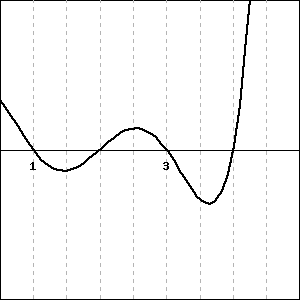
\includegraphics[scale=0.75]{wkst6img}
\end{center}

Using this graph (and estimating your answer whenever necessary), give the $x$-coordinate of a point where...

\begin{enumerate}

\item the \textbf{derivative} of $f(x)$ is negative:

\vfill

\item the \textbf{value} of $f(x)$ is negative:

\vfill

\item the \textbf{derivative} of $f(x)$ is smallest (most negative):

\vfill

\item the \textbf{derivative} of $f(x)$ is zero:

\vfill

\item the \textbf{derivative} of $f(x)$ is approximately the same as the \textbf{derivative} of $f(x)$ at $x=2.25$:

\vfill

\end{enumerate}

\newpage

\item Suppose that a ball is tossed straight up into the air. At time $t$ (the number of seconds after the ball was thrown), the height of the ball (in feet) is given by the function 
$$s(t)=64-16(t-1)^2.$$

\begin{enumerate}

\item Sketch the graph of $s(t)$ on the interval $[0,3]$. Label the points on the graph that correspond to when the ball was released, when the ball reaches its highest point, and when the ball lands.

\vspace{2in} 

\item Compute the value of $\frac{s(2.5)-s(1.5)}{2.5-1.5}$.

\vspace{1.65in}

\item What are the units on your answer to part (b)? \quad \rule{1.5in}{0.4pt}

\medskip
\newpage
\item Within the context of this problem (i.e., the motion of the ball), what is the meaning of the value that you found in (b)?

\vspace{1.85in}

\item The value that you found in (b) also represents the slope of a certain line. Draw this line on the graph you drew in part (a).

\medskip

\item Use a calculator to complete the following table:

\begin{center}
\begin{tabular}{c | c}
\text{Time interval $[a,b]$} & \text{$\frac{s(b)-s(a)}{b-a}$}\\
\hline\\[-15pt]
$[1.9, 2]$ & \\[14pt]
$[1.99, 2]$ & \\[14pt]
$[2, 2.1]$ & \\[14pt]
$[2, 2.01]$ & \\[14pt]
\end{tabular}
\end{center}

\item Using your completed table, estimate the \emph{instantaneous} velocity of the ball at time $t=2$.
 
 \vspace{0.75in}
 
\item Compute the derivative of the function $s(t)$ at $t = 2$. Compare this to your estimate above; is what you notice surprising?
\end{enumerate}

\newpage

  \item Compute the derivatives of the following functions at the indicated points:

    \begin{enumerate}
      \item $f(x) = x^2$ at $x = -1$.
        \vfill
      \item $f(x) = \dfrac{1}{x}$ at $x = 2$.
        \vfill
        \newpage
      \item $f'(1)$ where $f(x) = \sqrt{x + 3}$.
        \vfill
      \item $f'(1)$ where $f(x) = \dfrac{1}{x^2 + 1}$.
      \vfill
      \newpage
      \item $f'(1)$ where $f(x) = x^3 + x - 1$.
        \vfill
      \item $f'(0)$ where $f(x) = \sin(x)$.
        \vfill
    \end{enumerate}
\end{enumerate}

% Most people don't use these, so they are "commented out"
% by starting the lines with a "%"
%\begin{keywords}
%   \LaTeX, typesetting
%\end{keywords}

%\begin{AMS}
%   50C60, 18C25
%\end{AMS}

%%%%%%%%%%%%%%%%%%%%%%
% % Here is the start of the Text
%%%%%%%%%%%%%%%%%%%%%%
\end{document}
